% mixing properties, constrained czy restricted

\documentclass[oneside,a4paper]{article}
\usepackage[sectionbib,bibnewpage]{apacite}
\usepackage{amsmath}
\usepackage{bm}
\usepackage{float}
\usepackage{graphicx}
\usepackage{listings}

\title{The bhsdtr package: flexible bayesian inference for
  hierarchical or non-hierarchical equal variance normal Signal
  Detection Theory models with or without ratings.}

\begin{document}
\maketitle
\tableofcontents{}

\section{Abstract}

We describe a novel method of bayesian inference for hierarchical or
non-hierarchical equal variance normal Signal Detection Theory
models. The method is implemented as an open-source R package that
uses state of the art platform Stan for sampling from the posterior
distribution. Our method can accommodate binary responses as well as
additional ratings, the user can specify an arbitrary number of random
grouping factors, sensitivity and criteria parameters can be regressed
on additional predictors within the same model via intermediate
unconstrained parameters and the model can be extended by using an
automatically generated human-readable Stan code as a template. We
explain how our method improves other similar available methods, we
also provide an overview of the package and demonstrate the ease of
use and correctness of implementation by providing a real study data
analysis walk-through and by showing that the model successfully
recovers known parameter values when fitted to simulated data.

\section{Introduction}

Many tasks used in psychology studies are essentially classification
tasks. For example, in a memory study a test item may be either old or
new or in a perceptual study an object may either be a letter or a
digit. If a task requires classification it is always possible that
conclusions based on accuracy or percent correct are invalid because
the ability to discriminate between stimulus classes (i.e.,
sensitivity) is confounded with bias, which is the tendency to
classify stimuli as belonging to a particular class
\cite{GreenSwets66}. In principle, any effect that manifests itself in
the differences in classification accuracy may reflect differences in
sensitivity, bias or both. Signal Detection Theory provides a simple
and popular solution to this common and important problem. However,
SDT models are non-linear and variability in SDT parameters due to
factors such as participants or items has to be accounted for. When
effects of such factors are not accounted for in non-linear models
parameter estimates are biased and the associated uncertainty may be
underestimated.

We have created the \texttt{bhsdtr} package because in our opinion
available general purpose methods of fitting hierarchical SDT models
suffer from important limitations. The goal was to create a tool that
would be useful in a wide range of typical applications, that would
cover a broad spectrum of possible hierarchical structures defined on
SDT parameters and that would be relatively easy to use. We believe
that the \texttt{bhsdtr} package fulfills all of these goals. The
package is publicly available at
https://github.com/boryspaulewicz/bhsdtr, together with annotated R
code and data that was used to produce all the plots and perform all
the analyses described in this paper.

Our method is meant to be used by researchers already familiar with
Signal Detection Theory, hierarchical modelling and bayesian inference
so we begin by providing only a brief refreshment on certain issues in
SDT modelling. To those who do not yet possess the required expertise
we recommend \citeA{GelmanHill2007} for an introduction to bayesian
inference, hierarchical modelling and R and
\citeA{macmillan2004detection} for an introduction to SDT. Before we
go any further, however, a note on terminology seems in order.

In the context of hierarchical modelling factors such as participants,
items or replications are often referred to as groups, a naming
convention that we find confusing at times. For example, using this
terminology a single participant is both a group and a member of some
group, at the same time the term "group" is perhaps most strongly
associated with study conditions, as in "experimental group". In this
paper we use the term "sampled factor" instead, as it seems to capture
all the essential properties of such variables, i.e., the nominal
scale, the fact that values are sampled from a larger population and
are usually not of direct interest, as in "this is only a sample", and
that conclusions of statistical analysis are meant to apply to the
whole population of possible values (e.g., all the people or all the
items of a certain kind).

\section{Equal variance normal Signal Detection Theory model with
  additional criteria}

A generalization of the basic SDT model that we focus on here is shown
in Fig.~\ref{fig:1} below.

\begin{figure}[H]
  \centering
  \includegraphics[width=.8\linewidth]{plot_sdtr.pdf}
  \caption{Equal variance normal Signal Detection Theory model with
    additional criteria}
  \label{fig:1}
\end{figure}

The stimulus is assumed to give rise, by some unspecified cognitive
process, to unidimensional internal evidence value $s$ sampled from a
distribution that depends on the stimulus class. For historical
reasons the stimulus classess are often referred to as "noise" and
"signal" and task performance is described in terms of hits, correct
rejections, omissions and false alarms, but this terminology is
appropriate only when the model is applied to tasks that require
detection, which is by far not always the case. In the most widely
used version of the model the two evidence distributions are normal
with the same variance which is usually fixed at unity to make the
model identifiable. Sensitivity is represented by the distance $d'$
between the means of evidence distributions. Because normal
distributions are unbounded evidence is always ambiguous and a
criterion $c$ placed on the evidence axis has to be used to reach a
discrete decision. The location of the decision criterion represents
the direction and magnitude of bias. The generalized version of the
model shown in Fig.~\ref{fig:1} is applicable in studies where
participants are asked to rate their binary classification decisions
on a performance or stimulus related dimension, confidence being a
prime example. The ratings and binary classification decisions can be
provided together (e.g., "I am almost certain that it was a digit"),
or in an arbitrary order (ratings before or after the decision).

The ratings are accommodated by modelling combined response $y$, which
represents both the binary classification decision and rating. The
value of $y$ increases with the strength of evidence in favor of the
second stimulus class. For example, if confidence is rated on a
four-point scale, then $y = 1$ when the subject decides that the
stimulus belongs to the first class (e.g., an old item) with certainty
4, $y = 2$ corresponds to first stimulus class with certainty 3,
$y = 5$ corresponds to second stimulus class (e.g., a new item) with
certainty 1, and $y = 8$ corresponds to second stimulus class with
certainty 4. More formally, the subject is assumed to give response
$k$ if $k = \min \{i : s <= c_i\}$, where
$s \sim \text{Normal}(\mu, 1)$ and $\mu = -d'/2$ for the first
stimulus class and $\mu = d'/2$ for the second stimulus class, $K$ is
the number of possible responses and $c_i$ are the decision criteria,
with $c_0$ and $c_K$ fixed at $-\infty$ and $+\infty$ respectively.

When $K = 2$ (no ratings) the model always fits perfectly, because the
data and the model have the same dimensionality. This makes
generalization to the $K > 2$ case particularly important, as it is
only when $K > 2$ that formal assumptions of the model (e.g., equal or
unequal variance) can be tested\footnote{In contrast to formal
  assumptions the \emph{psychological interpretation} of SDT
  parameters can be tested even when ratings are not available, e.g.,
  by means of selective influence \cite{sternberg2001separate}}, often
by comparing the observed and the theoretical ROC
curves. % , although to the best of our knowledge there exists no direct
% test of the ROC curve shape.  Off course, depending on research
% questions these additional criteria can be of independent interest,
% as can be the ratio of evidence distribution variances or their
% functional form, but here we concentrate on more basic applications.

SDT is a non-linear model, and when non-linear models are used in
psychology studies researchers are usually interested in the
relationships between the free parameters of such models and certain
additional measured or manipulated variables. A good example in the
context of classification performance is the dependence of $d'$ (a
free parameter of a non-linear SDT model) on stimulus strength
(usually a manipulated variable). Also, in great many psychology
studies data have hierarchical structure, e.g., there are repeated
measures for each participant or item and participants or items are
only samples from the target population. It seems worthwhile to
explain why it is important that our method accommodates both kinds of
situations.

\subsection{Importance of hierarchical structure}

If data have hierarchical structure, as is typically the case when SDT
models are used, and assuming that the SDT model is true, it is only
when the requirement of accounting for variability due to subjects,
items or other such factors is met that the estimates of the average
(fixed) effects are guaranteed to be unbiased and the conclusions are
guaranteed to generalize to the target population.

A not so uncommon practice of analysing data aggregated over subjects,
items or other sampled factors represents an extreme case of ignoring
hierarchical data structure. Invalidity of this approach in the
context of SDT was clearly illustrated with results of simulational
studies by \citeA{morey2008problematic}, although strictly speaking it
requires such demonstrations only in order to make a point about a
specific case. Because SDT is a non-linear model, by definition
expected values of estimates of its parameters based on data
aggregated over sampled factors are not in general true population
averages. Such estimates are biased and inference about the target
population based on such estimates is simply not valid. To give a
concrete example, concider two unbiased participants, one with
$d' = 2$ and one with $d' = 4$. Their expected average accuracy is
given by $(\Phi(1) + \Phi(2)) / 2 = .91$, which corresponds to
$d' = 2.68$, whereas their true average $d'$ is $3$.

Aggregation is not the only way of ignoring hierarchical data
structure. Sometimes non-aggregated data are analyzed by using
separate estimates for every participant $\times$ item $\times$
condition combination but uncertainty due to subject or item effects
\emph{distributions} is not accounted for by means of hierarchical
model structure. In this case the conclusions, at least with respect
to the uncertainty in the estimates, are guaranteed to be valid only
for the given sample, not the target population. This is rarely, if
ever, the purpose of a study.

\subsection{Importance of including regression structure}

Another common source of problems is separation of estimation of
non-linear model parameters from regression analysis relating these
parameters to other measured or manipulated variables. When SDT
parameters are estimated separately for each subject and condition and
only later regressed on predictors of interest a number of additional
issues may arise.

Firstly, standard errors or credible intervals associated with
regression coefficients do not reflect the uncertainty in SDT
parameter estimates, because the latter are treated as mere data
points. This may lead to overly optimistic inference on regression
coefficients, since what this amounts to, among other things, is
ignoring part of the residual variance.

Secondly, including the regression part in the same model makes the
SDT parameter estimates dependent on the common regression structure
and so also on each other. This can improve their quality and affect
estimates of their uncertainty, just like assuming that random effects
are samples from a common distribution may improve their estimates by
making them dependent in the model.

Thirdly, the precision of parameter estimates often varies between
participants, items or conditions but when these estimates are treated
as mere data points in regression analysis no use is made of this
information. When regression structure is included in the same model
the regression coefficients are less influenced by the parameter
estimates that have lower precision.

\section{A critical summary of avaiable methods of bayesian inference
  for hierarchical SDT models}

To the best of our knowledge only two attempts at creating something
akin to the general purpose method of inference for hierarchical SDT
models with ratings can be found in literature. We will not consider
the ROC Toolbox \cite{Koen2016} or other similar tools here because as
of this writing these tools cannot be used to fit hierarchical SDT
models. The two available methods that can be used to fit hierarchical
SDT models are the Gibbs sampler proposed by
\citeA{morey2008problematic} and the Hierarchical Meta-d' model
(HMeta-d') proposed by \citeA{hmetad}. In our summary of these two
methods we mainly concentrate on two issues, namely the correctness of
hierarchical structure implementation and possibility to model SDT
parameters as dependent on additional variables.

\citeA{morey2008problematic} proposed a Gibbs sampling algorithm for
inference on hierarchical unequal variance normal SDT models with
ratings. A slightly modified version of the algorithm was later made
available as part of the \texttt{hbmem} R package. The authors adopted
what they called a fixed-criteria parametrization. Under this
parametrization the outermost criteria $\bm{c}_1$ and $\bm{c}_{K-1}$
are fixed at $0$ and $1$ respectively, while the remaining criteria
together with means and variances of the evidence distributions are
free to vary. The hierarchical part of evidence distribution means is
represented by additive independent normal effects of at most two
sampled factors which, following the authors, we label as subject and
item effects for convenience. However, the criteria are represented as
subject specific \emph{fixed}, not random effects. Items can have an
indirect and somewhat limited random effect on the criteria, because
they can have an effect on evidence distribution means by shifting
them independently. As the authors clarify, shifting both means by the
same amount in the same direction does not change the $d'$ but
simultaneously shifts all the criteria relative to the evidence
distributions. This allows an item to have the same effect on all the
criteria but it does not allow an item to have different effects on
different criteria. Random effects correlations are not accounted
for. Criteria are order-restricted, but the means of evidence
distributions are order-restricted only in the version implemented in
the \texttt{hbmem} package. SDT parameters can be regressed on
additional predictors to some extent by specifying a model
matrix. Lastly, because this is a Gibbs sampler, authors rely on
conjugate priors, including the problematic \cite{gelman2004prior}
inverse gamma prior placed on variances.

Fleming's \citeyear{hmetad} HMeta-d' model is a hierarchical version
of the meta-d' model \cite{maniscalco2012signal}, which in turn is a
generalization of the SDT model with additional criteria that allows
for a separate "meta-sensitivity" in order to account for possible
discrepancies between binary stimulus classification (referred to as
type 1 task) and a rating task (referred to as type 2 or
meta-cognitive task). We consider HMeta-d' here because it reduces to
the SDT model with ratings when type 1 and type 2 sensitivities are
equal. In HMeta-d' evidence distributions are normal with equal
variance. Normally distributed random effects of one factor are
allowed for sensitivities and parameters indirectly representing the
criteria, for lack of a better name from now on referred to as raw
criteria. The actual criteria are subject-specific sorted values of
unconstrained raw criteria and it is these unconstrained parameters,
not the actual criteria, that are given independent hierarchical
normal distributions representing variability due to subjects. Since
sorting is not injective the space of raw criteria is not isomorphic
to the space of actual criteria and each element of the raw criteria
vector can represent a value of any criterion, depending on the values
of other elements of the raw criteria vector. The model does not
account for possible correlations between random
effects. Sensitivities are represented as unrestricted scalars even
though they are non-negative by definition. Out of the box the code
provided by the author allows only for a very limited regression
structure to be placed on SDT parameters. Software implementation
relies on ready-made model specifications expressed in JAGS language
that are aimed at several simple types of experimental design (e.g.,
single subject or single group of subjects). The models can be fitted
using convenient MATLAB functions.

\section{Hierarchical Signal Detection Theory in unconstrained
  parameter space}

As we have already stressed, in a typical study both sensitivity and
criteria parameters have to be supplemented with hierarchical
structure for inference to be guaranteed to generalize to the target
population. In our critical summary of the two available methods we
have listed some reasons why we believe that without substantial
modifications neither method correctly addresses this issue. The main
reason why both methods fail in correctly specifying the hierarchical
structure on SDT parameters is that random effects are represented by
normal distributions but parameters are constrained, i.e.,
sensitivities are non-negative and criteria are ordered.

In the \texttt{bhsdtr} package sensitivities and criteria are derived
from unconstrained parameters by convenient isomorphisms. This is
easily achieved in case of sensitivity by deriving $d'$ from
$\delta = \ln(d')$ and modelling random effects on $d'$, if any, by
assuming that $\delta$ is normally distributed. Difficulties in
representing the hierarchical structure of the criteria stem from the
fact that even though each criterion considered in isolation is an
unconstrained parameter, the vector of all the criteria is ordered.
We propose to map the $R^{K-1}$ space, representing unconstrained
criteria, to the $K$ dimensional probability simplex space using the
softmax function and to map the simplex space to the ordered criteria
space by means of the inverse normal CDF. Specifically, assume that a
normal distribution is centered on the midpoint between the two
evidence distributions. The value of criterion $i$ is then given by:

\begin{align}
  \bm{c}_i &= \Phi^{-1}(\sum_{k = 1}^i(e^{\bm{\gamma}_k}) / \sum_{j=1}^K(e^{\bm{\gamma}_j}))
\label{eq:1}
\end{align}

\noindent where $\bm{\gamma} \in R^K$ with $\bm{\gamma}_K$ fixed at
$0$ for identifiability. The idea is illustrated in
Fig.~\ref{fig:2} below:

\begin{figure}[H]
  \centering
  \includegraphics[width=.8\linewidth]{plot.pdf}
  \caption{Mapping between unconstrained $\gamma$ vector and criteria}
  \label{fig:2}
\end{figure}

The mapping in Eq.~\ref{eq:1} is an isomorphism between the $R^{K-1}$
space and the space of $K-1$ ordered criteria vectors. Elements
$i = 1...K$ of the $\bm{\gamma}$ vector represent relative distances
between adjacent criteria because their exponents represent relative
magnitudes of areas under the normal curve delineated by the pairs of
adjacent criteria:
$e^{\bm{\gamma}_i} / e^{\bm{\gamma}_j} = (\Phi(\bm{c}_i) -
\Phi(\bm{c}_{i-1})) / (\Phi(\bm{c}_j) - \Phi(\bm{c}_{j-1}))$. When
$K=2$ only $\bm{\gamma}_1$ is free to vary and its value directly
represents the direction and magnitude of bias: $\bm{\gamma}_1$ is $0$
when the criterion is placed at the midpoint between the means of
evidence distributions, and the more negative (positive) it is the
more the criterion is placed to the left (right) of midpoint. Our
experience indicates that it is often a good idea to multiply all the
criteria by a value greater than $1$ which is equivalent to making the
mapping distribution in Eq.~\ref{eq:1} wider. This tends to even out
the values of $\bm{\gamma}$, especially when criteria are widely
spread as can happen for moderate to large $d'$ values. This feature
is implemented in the \texttt{bhsdtr} package by introducing a scaling
factor.

Once the $d'$ and $c$ are represented as derived from unconstrained
$\delta$ and $\gamma$ parameters the SDT model can be supplemented
with hierarchical linear regression structure. To avoid having to deal
with even more complicated index notation, below we have presented
only the simple case of one sampled factor.

\begin{align*}
  \bm{\delta} &= \bm{X}^{(\delta)} \bm{\beta}^{(\delta)} + \bm{Z}^{(\delta)} \bm{\theta}^{(\delta)} \\
  \bm{d'}_i &= e^{\bm{\delta}_i} \\
  \bm{\gamma}_{i,.} &= \bm{X}^{(\gamma)}_{i,.} \bm{\beta}^{(\gamma)} + \bm{Z}^{(\gamma)}_{i,.}
                      \bm{\theta}^{(\gamma)} \\
  \bm{c}_{i,k} &= s \ \Phi^{-1}(\sum_{l = 1}^i(e^{\bm{\gamma}_{i,l}}) /
                 \sum_{m=1}^K(e^{\bm{\gamma}_{i,m}})) \\
  p(\bm{y}_i = k|\bm{stim}_i = 1) &= \Phi(\bm{c}_{i,k} + \bm{d'}_i / 2) - \Phi(\bm{c}_{i,k-1} + \bm{d'}_i / 2) \\
  p(\bm{y}_i = k|\bm{stim}_i = 2) &= \Phi(\bm{c}_{i,k} - \bm{d'}_i / 2) - \Phi(\bm{c}_{i,k-1} - \bm{d'}_i / 2)
\end{align*}

\noindent Here $i$ is the observation number, $\bm{X}$ is the fixed
effects model matrix for the respective parameter, $\bm{Z}$ is the
random effects model matrix, $\bm{\beta}$ and $\bm{\theta}$ are the
fixed and random effects, $\bm{c}_{i,k}$ is the $k$-th criterion for
the $i$-th observation, $s$ is the criteria scaling factor, and
$\bm{y}$ is the combined response. Note that $\bm{d'}_i$ is a scalar,
but $\bm{\gamma}_{i,.}$ is in general a vector and so
$\bm{\beta}^{(\gamma)}$ and $\bm{\theta}^{(\gamma)}$ are matrices. The
$j$-th rows of the $\bm{\beta}^{(\gamma)}$ and
$\bm{\theta}^{(\gamma)}$ matrices represent fixed and random effects
for the $j$-th element of the $\bm{\gamma}$ vector.

Following \citeA{sorensen2015bayesian} we make use of the Cholesky
decomposition of the correlation matrices because it improves
efficiency and admits a convenient prior on random effects'
correlations:

\begin{align*}
  \text{vectorized}(\bm{\theta}^{(\gamma)}) &= \text{diag}(\bm{\tau}^{(\gamma)}) \bm{L}^{(\gamma)} \bm{z}^{(\gamma)} \\
  \bm{\theta}^{(\delta)} &= \text{diag}(\bm{\tau}^{(\delta)}) \bm{L}^{(\delta)} \bm{z}^{(\delta)} \\
  \bm{z}^{(\delta)}_i &\sim \text{Normal}(0, 1) \\
  \bm{z}^{(\gamma)}_j &\sim \text{Normal}(0, 1)
\end{align*}

\noindent where $\bm{\tau}$ is a vector of standard deviations of
random effects and $\bm{L}$ is the Cholesky decomposition of the
correlation matrix, i.e., $\bm{C} = \bm{L} \bm{L}'$. This way
$\bm{\theta}$ is multivariate normal with covariance matrix
$\text{diag}(\bm{\tau}) \bm{L}$.

We use weakly informative proper priors because they provide
regularization and help stabilize computation. Fixed effects
($\bm{\beta}^{(\delta)}$ and $\bm{\beta}^{(\gamma)}$) are given
independent normal priors, random effects standard deviations
($\bm{\tau}^{(\delta)}$ and $\bm{\tau}^{(\gamma)}$) are given
independent half-Cauchy priors as recommended by
\citeA{gelman2004prior} and each $\bm{L}$ is given an independent lkj
prior:

\begin{align*}
  \bm{\beta}^{(\delta)}_i &\sim \text{Normal}(\bm{\mu}^{(\delta)}_i, \bm{\sigma}^{(\delta)}_i) \\
  \bm{\beta}^{(\gamma)}_{k,l} &\sim \text{Normal}(\bm{\mu}^{(\gamma)}_{k,l}, \bm{\sigma}^{(\gamma)}_{k,l}) \\
  \bm{\tau}^{(\delta)}_i &\sim \text{half-Cauchy}(0, \bm{\zeta}^{(\delta)}_i) \\
  \bm{\tau}^{(\gamma)}_{k,l} &\sim \text{half-Cauchy}(0, \bm{\zeta}^{(\gamma)}_{k,l}) \\
  \bm{L}^{(\delta)} &\sim \text{lkj}(\nu^{(\delta)}) \\
  \bm{L}^{(\gamma)} &\sim \text{lkj}(\nu^{(\gamma)}) \\
\end{align*}

\subsection{Specifying prior distributions}

Specifying the priors on sensitivity effects does not pose any special
difficulties. Sensitivity of an unbiased classifier given percent
correct is given by $2 \Phi^{-1}(\text{pc})$. When both stimulus
classes are equally likely the greater the bias the lower the accuracy
meaning that unbiased sensitivity represents the lower bound on
sensitivity given percent correct. Let us assume that a great majority
of subjects are expected to achieve percent correct within the $.51$
to $.99$ range with negligible bias. Since
$\ln(2\Phi^{-1}(.51)) = -2.99$ and $\ln(2 \Phi^{-1}(.99)) = 1.54$ a
reasonable weakly informative prior on delta is normal with mean
$(1.54 - 2.99) / 2$ and standard deviation $(1.54 + 2.99) / 2$ which
is the default prior on delta effects in the \texttt{bhsdtr}
package.

Specifying priors on the criteria can be challenging because of the
ordering restriction. In addition, complexity of mapping in
Eq.~\ref{eq:1} makes it difficult to reason about the priors on
$\bm{\gamma}$ in terms of the criteria. By default in the
\texttt{bhsdtr} package each entry in $\bm{\sigma}^{(\gamma)}$ and
$\bm{\zeta}^{(\gamma)}$ matrices is set to $\ln(100)$ and the criteria
scaling factor is fixed at 2. The meaning of $\ln(100)$ depends on
model matrix parametrization to some degree, but usually it means that
a priori areas under the mapping distribution between adjacent
criteria may easily differ from the area between criterion $K-1$ and
$K$ by a factor of 100 but differences by a factor of $2 \ln(100)$ or
more are highly unlikely. Off course, when in doubt it is a good idea
to perform some sort of sensitivity analysis, remembering that strong
sensitivity to priors indicates that the study may be underpowered.

The prior on random effects standard deviations is parametrized by
$\bm{\zeta}$, which represents half-width at half-maximum of the
half-Cauchy distribution. In our opinion a not-unreasonable starting
point is to set $\bm{\zeta}$ at the value that is greater or equal to
the most likely value of the random effects standard deviation.

By default $\nu^{(\delta)} = \nu^{(\gamma)} = 1$ implying a uniform
prior on random effects correlation matrices. Because the greater the
value of $\nu$ the more emphasis is put on zero off-diagonal
correlations the researcher can force the correlations to be near-zero
by choosing large $\nu$ value.

\section{Overview of the software implementation}

We have chosen the Stan modelling language \cite{carpenter2016stan}
because it uses state-of-the-art adaptive Hamiltonian Monte Carlo
sampling algorithm which often handles high-dimensional correlated
posteriors better than the Gibbs sampler. The \texttt{bhsdtr} package
is essentially a collection of documented functions. The
\texttt{aggregate\_responses} function serves to aggregate the data as
much as possible for efficiency, but without distorting the
hierarchical structure. The \texttt{make\_stan\_model} function
creates the model code based on the provided model formulae for random
effects. The Stan code produced by the \texttt{make\_stan\_model}
function can be fitted as is or modified by the user if needed, e.g.,
to change the prior distributions or drop the equal variance
assumption. The \texttt{make\_stan\_data} function creates regression
model matrices and other data structures required by the model created
with the \texttt{make\_stan\_model} function. Finally, the
\texttt{plot\_sdt\_fit} function can be used to assess the model fit
visually. This function creates publication-ready ROC curve plots or
response distribution plots with posterior predictive intervals
calculated for the chosen $\alpha$ level.

\subsection{Usage example: installing the package and testing the
  model on real data}

In order to make full use of the \texttt{bhsdtr} package functionality
three non-standard R packages are required, namely \texttt{rstan},
\texttt{plyr} and \texttt{ggplot2}. We recommend using the
\texttt{devtools} package to install the \texttt{bhsdtr} package
directly from the github repository. This will also automatically
install any missing required packages:

\begin{lstlisting}{language = R}
  devtools::install_git('boryspaulewicz/bhsdtr')
  library(bhsdtr)
\end{lstlisting}

We tested our method on the \texttt{gabor} dataset that is part of the
\texttt{bhsdtr} package. The \texttt{gabor} dataset comes from an
unpublished study in which on each trial participants had to classify
the briefly presented gabor patch as either oriented to the left or to
the right using the arrow keys. The participants were also asked to
rate the stimuli on a 4 point Perceptual Awareness Scale
\cite{ramsoy2004introspection} presented at the bottom of the
screen. The gabor patch was immediately followed by a mask. The PAS
ratings ranged from "no experience" to "absolutely clear image" and
were provided either before (RD condition) or after (DR condition)
pressing the arrow keys. On each trial the gabor patch was equally
likely to be presented for 32ms or 64ms. Decision-rating order was a
between-subject variable and gabor patch presentation duration was a
within-subject variable. There were 47 participants and 48 trials per
condition.

We will now explain how to perform some of the essential steps of a
typical data analysis process, which at the very least usually
involves preparing the data, creating the model code, fitting the
model, assessing the fit, and possibly converting the unconstrained
$\gamma$ and $\delta$ parameters to $d'$ and $c$.

\subsubsection{Step 1: preparing the data}

In the study in question the response was originally encoded as
accuracy and rating, so the first step was to create an appropriate
response variable using the \texttt{combined\_response} function. This
function needs three variables, one encoding the stimulus class, one
encoding the rating (as an integer) and one encoding decision
accuracy. This step is required only if ratings are available and the
combined response variable is not already present in the data. In the
$K=2$ case the combined response variable is simply the binary
classification decision.

\begin{lstlisting}{language=R}
  gabor$resp = combined_response(gabor$stim, 
                                 gabor$rating, 
                                 gabor$acc)
\end{lstlisting}

Next, the data was aggregated by computing combined response counts,
but only to the extent that preserved all the participant effects. The
\texttt{aggregate\_responses} function that does exactly this requires
as arguments a data frame containing all relevant variables, a name of
the stimulus class variable, a name of the combined response variable
and a vector of names of all variables that are to be preserved in a
resulting aggregated dataset, i.e., those encoding sampled factors and
those representing independent variables used in the regression part
of the model:

\begin{lstlisting}{language=R}
adata = aggregate_responses(gabor, 'stim', 'resp', 
                            c('id', 'duration', 'order'))  
\end{lstlisting}

The main purpose of the aggregation step is to improve the efficiency
of sampling from the posterior distribution. When the data are
aggregated in this way the likelihood for each condition $\times$
participant combination has to be computed only once rather than as
many times as there are trials per condition per participant. Note
that if there are other sampled factors present in the data (e.g.,
items, replications, etc.) then these factors have to be specified at
this stage as well to preserve hierarchical structure. The
\texttt{aggregate\_responses} function creates a list with three
components. The \texttt{data} component is a data frame containing
additional preserved variables, the \texttt{stimulus} component is the
stimulus class variable and the \texttt{counts} component is a matrix
of counts with $K$ columns, where $K$ is the highest possible combined
response.

\subsubsection{Step 2: creating the model code}

The model is fitted using the \texttt{stan} function from the
\texttt{rstan} package which needs a special list of data structures
used by the model as well as a model specification expressed in the
Stan language. Every SDT model has some fixed effects structure, since
even when there are no predictors the model parameters can be
expressed as regressed on a vector of ones (i.e., an
intercept). However, many models also have a hierarchical structure
and, if that is the case, this hierarchical structure has to be
specified when using the \texttt{make\_stan\_model} function. This is
done by providing a list of lists of R model formulae. Each list of
model formulae is composed of at least three elements and specifies
correlated random effects of one sampled factor. The element named
\texttt{group} specifies the sampled factor and the elements named
\texttt{delta} and \texttt{gamma} specify which effects are assumed to
vary between the levels of this sampled factor. When
\texttt{make\_stan\_model} is used without any arguments it specifies
the SDT model without any random effects. Fixed effects model matrices
are specified by providing a list with at least two model formulae,
named \texttt{delta} and \texttt{gamma}, to the
\texttt{make\_stan\_data} function, described later in this
paper. Non-default priors can be specified by adding optional elements
to the random and fixed effects specification lists, as described in
the \texttt{make\_stan\_data} function documentation.

In the study in question there was only one sampled factor (id) which
represents participants. Because duration was a within-participant
variable in principle its effect could vary between participants for
all the SDT parameters. However, preliminary data analysis indicated
that the barely noticeable 32ms difference in duration seemed to
affect only the sensitivity. Thus, it was assumed that duration
affects only the $\delta$ parameter and that this effect may vary
between participants:

\begin{lstlisting}{language=R}
fixed = list(delta = ~ -1 + duration:order, 
             gamma = ~ order)
random = list(list(group = ~ id, 
              delta = ~ -1 + duration, 
              gamma = ~ 1))
model = make_stan_model(random)
\end{lstlisting}

The \texttt{make\_stan\_data} function creates fixed and random effect
model matrices based on the respective model formulae using dummy
contrast coding. Note that the implicit intercept was suppressed for
the $\delta$ model matrix. This way $\delta$ was estimated for every
duration $\times$ order condition\footnote{R uses dummy contrast
  coding by default}. The resulting separate intercepts and slopes
parametrization makes it easier to calculate arbitrary contrasts based
on the posterior samples. A more standard parametrization was used for
the $\gamma$ parameter, because it was initially assumed that criteria
depend only on order and so there was only one contrast of interest
for every element of the $\gamma$ vector. On the other hand even in
such case the separate intercepts and slopes parametrization may be
more convenient if the researcher is interested in the actual
criteria. It is perhaps worth emphasising how the separation of
$\delta$ and $\gamma$ regression structures makes it possible to test
a broad class of linear models representing the dependence of
sensitivity and criteria on additional variables.

\subsubsection{Step 3: fitting the model}

A separate data structure used by the Stan sampler has to be created
using the \texttt{make\_stan\_data} function. The obligatory arguments
to this function are the aggregated data object created by
\texttt{aggregate\_responses} function and fixed effects
specification. Because in our example study duration was a
within-subject variable here we also provide the random effects
specification. Importantly, if random effects are modelled the same
random effects specification has to be provided to the
\texttt{make\_stan\_model} and \texttt{make\_stan\_data} functions.

\begin{lstlisting}{language=R}
sdata = make_stan_data(adata, fixed, random)
\end{lstlisting}

Finally, a vector of names of parameters of interest has to be
specified when calling the \texttt{stan} function:

\begin{lstlisting}{language=R}
fit = stan(model_code = model,
           data = sdata,
           pars = c('delta_fixed', 'gamma_fixed',
                    'delta_sd_1', 'gamma_sd_1',
                    'delta_random_1', 'gamma_random_1',
                    'Corr_delta_1', 'Corr_gamma_1',
                    'counts_new'),
           iter = 8000,
           chains = 4)
\end{lstlisting}

Note that since more than one sampled factor is allowed the names of
parameters defining the hierarchical part are indexed (e.g.,
\texttt{delta\_sd\_1}, \texttt{delta\_random\_1},
\texttt{Corr\_delta\_1}). The name \texttt{counts\_new} refers to the
posterior predictive samples that are required by the
\texttt{plot\_sdt\_fit} function, names starting with \texttt{Corr}
refer to random effects correlation matrices.

\subsubsection{Step 4: assessing the model fit}

Four chains of 8000 iterations each were run simultaneously and the
first half of the posterior samples serving as a warm-up period for
tuning the parameters of the sampling algorithm was discarded. Part of
the resulting stan output is presented in Table~\ref{tab:fitsum}
below.

\begin{table}[H]
\caption{Model fit summary statistics}
\label{tab:fitsum}
\begin{tabular}{rrrrrrrr}
  \hline
  & mean & $SE_{mean}$ & $SD$ & $2.5\%$ & $97.5\%$ & Effective samples & $\hat{R}$ \\ 
  \hline
  delta\_fixed[1] & -0.10 & 0.00 & 0.15 & -0.41 & 0.18 & 4626 & 1.00 \\ 
  delta\_fixed[2] & 1.12 & 0.00 & 0.09 & 0.95 & 1.29 & 4764 & 1.00 \\ 
  delta\_fixed[3] & -0.39 & 0.00 & 0.20 & -0.80 & -0.03 & 5427 & 1.00 \\ 
  delta\_fixed[4] & 1.28 & 0.00 & 0.11 & 1.06 & 1.50 & 5464 & 1.00 \\ 
  gamma\_fixed[1,1] & -0.14 & 0.00 & 0.06 & -0.27 & -0.02 & 2925 & 1.00 \\ 
  gamma\_fixed[1,2] & -0.22 & 0.00 & 0.10 & -0.42 & -0.01 & 8199 & 1.00 \\ 
  gamma\_fixed[2,1] & -0.70 & 0.00 & 0.18 & -1.05 & -0.35 & 3060 & 1.00 \\ 
  gamma\_fixed[2,2] & 0.49 & 0.00 & 0.29 & -0.06 & 1.04 & 3452 & 1.00 \\ 
  gamma\_fixed[3,1] & -0.54 & 0.00 & 0.22 & -0.96 & -0.11 & 3103 & 1.00 \\ 
  gamma\_fixed[3,2] & 0.83 & 0.01 & 0.35 & 0.14 & 1.51 & 3086 & 1.00 \\ 
  gamma\_fixed[4,1] & 0.28 & 0.00 & 0.25 & -0.20 & 0.76 & 3090 & 1.00 \\ 
  gamma\_fixed[4,2] & 0.42 & 0.01 & 0.40 & -0.37 & 1.22 & 3291 & 1.00 \\ 
  gamma\_fixed[5,1] & -0.21 & 0.01 & 0.30 & -0.80 & 0.37 & 3440 & 1.00 \\ 
  gamma\_fixed[5,2] & 0.83 & 0.01 & 0.48 & -0.10 & 1.78 & 3637 & 1.00 \\ 
  gamma\_fixed[6,1] & -0.77 & 0.00 & 0.24 & -1.23 & -0.31 & 3378 & 1.00 \\ 
  gamma\_fixed[6,2] & 0.80 & 0.01 & 0.38 & 0.05 & 1.56 & 3316 & 1.00 \\ 
  gamma\_fixed[7,1] & -0.32 & 0.00 & 0.16 & -0.64 & 0.01 & 3346 & 1.00 \\ 
  gamma\_fixed[7,2] & 0.42 & 0.00 & 0.28 & -0.11 & 0.98 & 3333 & 1.00 \\ 
  delta\_sd\_1[1] & 0.66 & 0.00 & 0.11 & 0.48 & 0.90 & 6373 & 1.00 \\ 
  delta\_sd\_1[2] & 0.44 & 0.00 & 0.05 & 0.35 & 0.56 & 5463 & 1.00 \\ 
  gamma\_sd\_1[1] & 0.16 & 0.00 & 0.08 & 0.02 & 0.31 & 2071 & 1.00 \\ 
  gamma\_sd\_1[2] & 0.82 & 0.00 & 0.11 & 0.62 & 1.06 & 5852 & 1.00 \\ 
  gamma\_sd\_1[3] & 1.08 & 0.00 & 0.12 & 0.86 & 1.33 & 4293 & 1.00 \\ 
  gamma\_sd\_1[4] & 1.27 & 0.00 & 0.14 & 1.03 & 1.57 & 3723 & 1.00 \\ 
  gamma\_sd\_1[5] & 1.55 & 0.00 & 0.17 & 1.24 & 1.91 & 4297 & 1.00 \\ 
  gamma\_sd\_1[6] & 1.18 & 0.00 & 0.13 & 0.95 & 1.47 & 4348 & 1.00 \\ 
  gamma\_sd\_1[7] & 0.78 & 0.00 & 0.10 & 0.60 & 1.00 & 4399 & 1.00 \\ 
  Corr\_delta\_1[1,1] & 1.00 & 0.00 & 0.00 & 1.00 & 1.00 & 16000 &  \\ 
  Corr\_delta\_1[1,2] & 0.76 & 0.00 & 0.10 & 0.52 & 0.91 & 3871 & 1.00 \\ 
  Corr\_delta\_1[2,1] & 0.76 & 0.00 & 0.10 & 0.52 & 0.91 & 3871 & 1.00 \\ 
  Corr\_delta\_1[2,2] & 1.00 & 0.00 & 0.00 & 1.00 & 1.00 & 15199 & 1.00 \\ 
  Corr\_gamma\_1[1,1] & 1.00 & 0.00 & 0.00 & 1.00 & 1.00 & 16000 &  \\ 
  Corr\_gamma\_1[1,2] & -0.20 & 0.01 & 0.27 & -0.66 & 0.39 & 840 & 1.00 \\ 
  Corr\_gamma\_1[1,3] & -0.17 & 0.01 & 0.28 & -0.67 & 0.41 & 820 & 1.01 \\ 
  Corr\_gamma\_1[1,4] & -0.04 & 0.01 & 0.28 & -0.56 & 0.51 & 840 & 1.00 \\ 
  Corr\_gamma\_1[1,5] & -0.06 & 0.01 & 0.28 & -0.60 & 0.49 & 836 & 1.00 \\ 
  Corr\_gamma\_1[1,6] & -0.27 & 0.01 & 0.27 & -0.75 & 0.32 & 838 & 1.00 \\ 
  Corr\_gamma\_1[1,7] & -0.19 & 0.01 & 0.28 & -0.69 & 0.39 & 871 & 1.01 \\ 
  Corr\_gamma\_1[2,1] & -0.20 & 0.01 & 0.27 & -0.66 & 0.39 & 840 & 1.00 \\ 
  Corr\_gamma\_1[2,2] & 1.00 & 0.00 & 0.00 & 1.00 & 1.00 & 16000 & 1.00 \\ 
  Corr\_gamma\_1[2,3] & 0.58 & 0.00 & 0.13 & 0.29 & 0.79 & 3716 & 1.00 \\ 
  Corr\_gamma\_1[2,4] & 0.39 & 0.00 & 0.15 & 0.06 & 0.65 & 2806 & 1.00 \\ 
  Corr\_gamma\_1[2,5] & 0.22 & 0.00 & 0.16 & -0.11 & 0.52 & 2712 & 1.00 \\ 
  Corr\_gamma\_1[2,6] & 0.46 & 0.00 & 0.14 & 0.17 & 0.70 & 3968 & 1.00 \\ 
  Corr\_gamma\_1[2,7] & 0.80 & 0.00 & 0.09 & 0.60 & 0.93 & 5171 & 1.00 \\ 
  \dots{} & \dots{} & \dots{} & \dots{} & \dots{} & \dots{} & \dots{}
                                                                       & \dots{} \\
  \hline
\end{tabular}
\end{table}

As can be seen, the chains exhibited good mixing properties given the
complexity of the model and seemed to have reached apparent
convergence: there were enough effective samples of fixed effect
parameters to estimate $95\%$ credible intervals well and none of the
Gelman-Rubin $\hat{R}$ statistics crossed the conventional $1.01$
threshold suggesting negligible sensitivity to initial values.

Fig.~\ref{fig:6} and \ref{fig:7} below contain normal
quantile-quantile plots of random effects showing that normally
distributed random $\delta$ and $\gamma$ effects seem to be good
candidates for representing variability in sensitivities and criteria
due to sampled factors.

\begin{figure}[H]
  \centering
  \includegraphics[width=.8\linewidth]{delta_qq_plot.pdf}
  \caption{Normal quantile-quantile plots of $\delta$ random effects}
  \label{fig:6}
\end{figure}

\begin{figure}[H]
  \centering
  \includegraphics[width=.8\linewidth]{gamma_qq_plot.pdf}
  \caption{Normal quantile-quantile plots of $\gamma$ random effects}
  \label{fig:7}
\end{figure}

Even when stan output summary does not indicate any obvious sampler
convergence issues before drawing any further conclusions the
researcher should first check if the model fits the data. We recommend
using the \texttt{plot\_sdt\_fit} function for that purpose:

\begin{lstlisting}{language = R}
plot_sdt_fit(fit, adata, c('order', 'duration')))
\end{lstlisting}

This function needs at least three agruments; a stanfit object, an
aggregated data list produced by the \texttt{aggregate\_responses}
function that was used to produce the stanfit object and a vector of
names of variables that define how the data will be partitioned before
plotting. Even though we highly recommend assessing the fit at the
individual level we did not include the participant identification
number in the list of conditioning variables because the resulting
plot would take up too much space. As can be seen in Fig.~\ref{fig:3}
showing the ROC curves produced by the code above the model seemed to
fit the data well in all but one condition (decision after rating,
64ms duration) where three out of seven relevant\footnote{The point in
  the upper-right corner of the ROC curve is always in the $(1,1)$
  position} points were outside the two-dimensional 95\% posterior
predictive regions.

\begin{figure}[H]
  \centering
  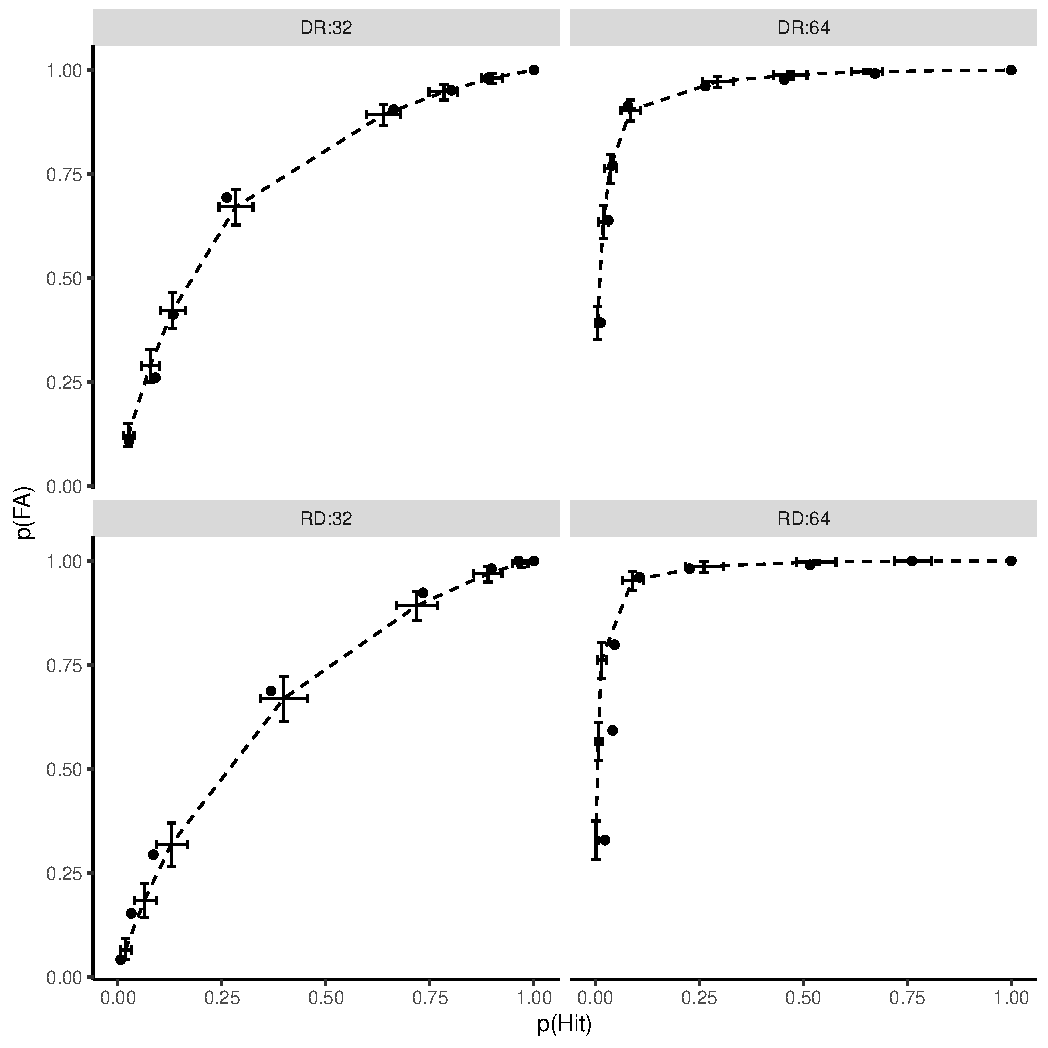
\includegraphics[width=.8\linewidth]{roc_fit.pdf}
  \caption{ROC curve fit}
  \label{fig:3}
\end{figure}

Another way to assess the model fit visually is by inspecting the
conditional response distributions ($p(y|stim)$) shown in
Fig.~\ref{fig:4} which was also created using the
\texttt{plot\_sdt\_fit} function.

\begin{figure}[H]
  \centering
  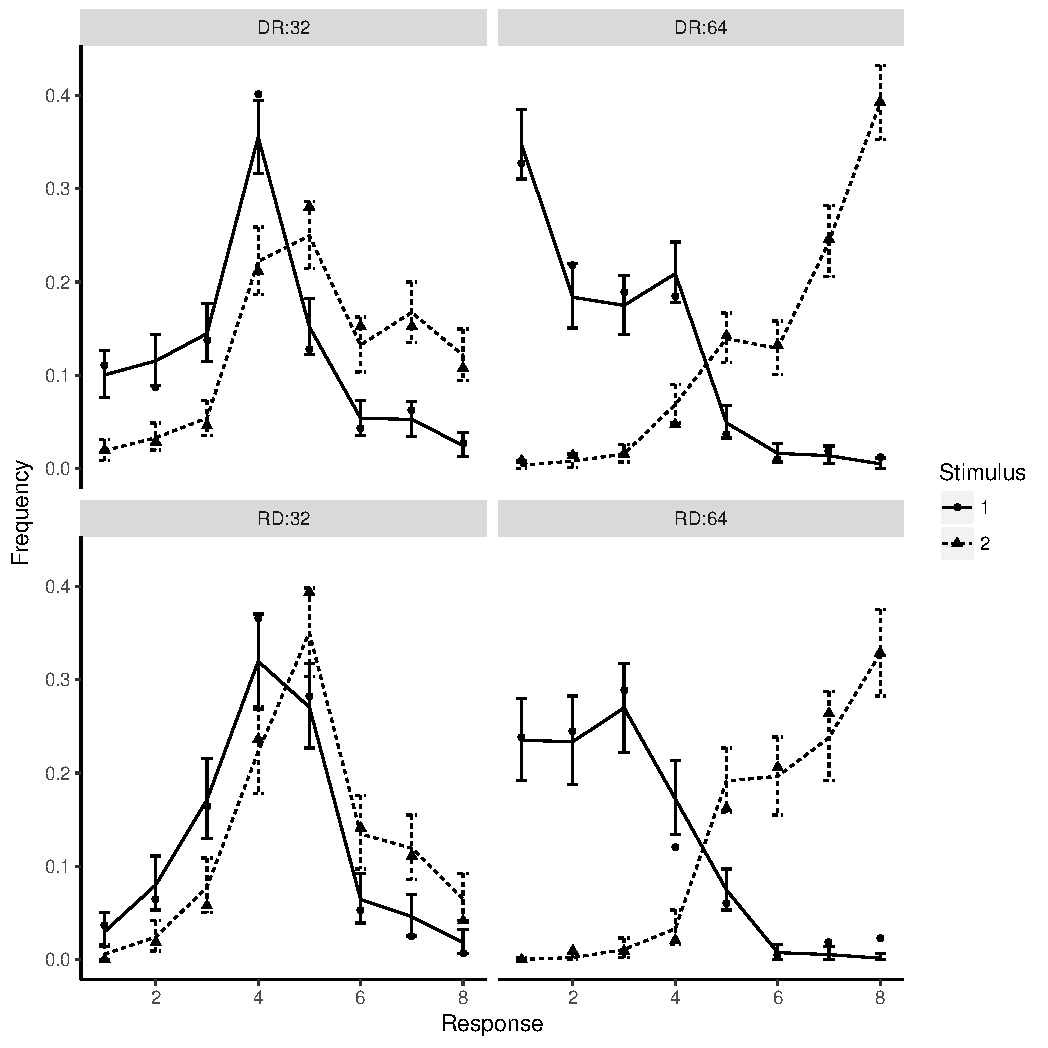
\includegraphics[width=.8\linewidth]{response_fit.pdf}
  \caption{Response distribution fit}
  \label{fig:4}
\end{figure}

This kind of plot can sometimes be informative about the reasons why
the model does not fit the data. In this particular case the plot
seems to suggest that it may be a good idea to inspect the fit at the
individual level and see if there are some participants with unusual
$p(y|stim=1)$ distributions in the RD $\times$ 64ms condition. On the
other hand it is also possible that the lack of fit was mainly a
consequence of the assumption that duration had zero effect on
$\bm{\gamma}$ or maybe the model is simply incorrect and more
substantial modifications are necessary.

\subsubsection{Step 5: converting unconstrained $\delta$ and $\gamma$
  parameters to sensitivities and criteria}

The posterior $\delta$ and $\gamma$ samples have to be transformed in
order to work with $d'$ and $c$ parameters. This is straightforward
only when fixed effects represent separate conditions, not the
differences between conditions or the regression slopes. In our
example, because separate intercepts and slopes parametrization was
used for the $\delta$ fixed effects model matrix all four
\texttt{delta\_fixed} parameters can easily be transformed to
sensitivities by applying the logarithm function to the posterior
samples. It is important to remember that the $\delta$ to $d'$
conversion should usually be done first, before applying any other
transformations to the samples, for example, the logarithm of point
and interval $\delta$ estimate is not equal to the point and interval
$d'$ estimate.

In case of the \texttt{gamma\_fixed} matrix the first column (the
intercept) corresponds to the values of the $\bm{\gamma}$ vector
\emph{in} the DR condition but the second column corresponds to
\emph{the effect} of the order variable on the $\bm{\gamma}$
vector. For this reason in this particular case posterior criteria
samples can be obtained using the \texttt{gamma\_to\_crit} function
only for the first column of the \texttt{gamma\_fixed} matrix.

\subsection{Testing the model on simulated data}

To test if the model correctly recovers known parameter values we have
simulated the data from a hypothetical exact replication of the
previously described experiment using point estimates from the
previous fit as known realistic parameter values. Mixing performance
and apparent convergence were similar as in the real data case. All
the model parameters were correctly recovered in a sense that the true
values were outside the 95\% credible intervals no more than 5\% of
the time.

For illustration purposes the SDT model that differed from the true
model only in that it did not have the hierarchical structure
representing participant effects was fitted to the same simulated
dataset. Since the model was much simpler and the data consisted of
only eight vectors of response counts apparent convergence was quickly
reached and chain mixing was excellent.

Point and interval estimates of fixed effects based on both models are
compared in Fig.~\ref{fig:5} below. The estimates were centered at the
true values to simplify the presentation. As can be seen, the true
model correctly recovered known parameter values, but estimates based
on the non-hierarchical model were clearly biased; $95\%$ credible
intervals were not only about three times shorter on average but also
failed to contain most of the true values.

\begin{figure}[H]
  \centering
  \includegraphics[width=.8\linewidth]{true_vs_nonhier.pdf}
  \caption{Comparison of point and interval posterior estimates based
    on the true and simplified non-hierarchical models}
  \label{fig:5}
\end{figure}

However, as can be seen on Fig.~\ref{fig:8} below in this case the
observed ROC curves seemed to fit the simplified model's predictions
quite well, giving a false impression of model validity.

\begin{figure}[H]
  \centering
  \includegraphics[width=.8\linewidth]{roc_sim_aggr_fit.pdf}
  \caption{ROC curve fit for the non-hierarchical model}
  \label{fig:8}
\end{figure}

\section{Concluding remarks}

The great importance of SDT to psychology stems from the fact that
given some fairly weak assumptions about the underlying decision
process it promises to deconfound sensitivity from bias in arbitrary
classification tasks. To the best of our knowledge at present the
\texttt{bhsdtr} package provides the only method of bayesian inference
for SDT models with or without ratings that can be recommended as a
default choice in typical applications. Our method allows for great
flexibility that requires minimal input from the user. Parametrization
forces sensitivities to be non-negative and criteria to be ordered
while the isomorphisms between unconstrained $\delta$ and $\gamma$ and
derived $d'$ abd $c$ parameters ensure that hierarchical structure is
valid. There is no limit to the number of sampled factors except for
the one imposed by available computational resources, correlations of
random effects of the same sampled factor are accounted for, all the
SDT parameters can be modelled by linear regression within the same
model and all the effects on all the SDT parameters estimable within
the levels of sampled factors can have associated correlated random
effects. In case a need arises to relax a built-in restriction
experienced users can extend the model in arbitrary ways by using
automatically generated human-readable Stan model code as a
template. We hope that researchers with basic understanding of Signal
Detection Theory, bayesian inference and hierarchical modelling will
find our package useful and adopt it as a method of analysis of
classification performance in their future studies. In the near future
we are planning to extend the package by relaxing the equal variance
assumption and adding the ability to fit other generalizations of SDT,
such as the meta-d' model, that allow for different information to be
used by classification decision and rating.

\bibliography{/home/borys/cs/literatura}
\bibliographystyle{apacite}
\end{document}
